\chapter{Analýza existujúcich rezervačných systémov a špecifikácia požiadaviek}\label{chap:analyza}
Táto kapitola analyzuje súčasný stav organizácie konzultačných hodín na Fakulte informačných technológií VUT, identifikuje nedostatky existujúcich riešení a na ich základe špecifikuje požiadavky na novú mobilnú aplikáciu „Office Hours".

\section{Analýza existujúcich riešení}
\subsection{Systém Wiki@Merlin}
Základným využívaným nástrojom na Fakulte informačných technológií VUT v Brne je systém Wiki@Merlin\footnote{Wiki@Merlin – webový wiki systém určený na zdieľanie informácií týkajúcich sa školských projektov a rôznych návodov užitočných v rámci štúdia na FIT VUT. Dostupné na: \url{https://merlin.fit.vut.cz/wiki/index.php/Wiki@Merlin}}, bežiaci na rovnomennom fakultnom serveri. Ide o platformu, ktorá primárne slúži na zdieľanie študijných materiálov, návodov a organizáciu predmetov. Mnohí vyučujúci tento systém historicky adaptovali aj na vypisovanie a správu konzultačných hodín. Kontrola prístupu je zabezpečená na úrovni celého systému. Pred zobrazením či úpravou stránky so slotmi systém vyžaduje prihlásenie pomocou školského prihlasovacieho mena a hesla.

Proces rezervácie v tomto systéme spočíva v manuálnej úprave textového dokumentu, kde študenti dopisujú svoje mená do predpripravenej tabuľky alebo zoznamu pomocou špecifickej wiki syntaxe. Tento prístup so sebou prináša dva zásadné problémy. Prvým je výrazný diskomfort pri používaní na mobilných zariadeniach. Používateľské rozhranie systému nie je plne prispôsobené pre mobilné zariadenia, čo pri úprave textu na malom displeji smartfónu vyžaduje neustále približovanie, posúvanie obrazovky a sťažuje orientáciu vo wiki syntaxi stránky.

Druhým problémom je absencia ochrany jednotlivých rezervácií. Keďže systém nerozlišuje vlastníka konkrétneho riadku v texte, každý používateľ s prístupom k úprave stránky môže (či už omylom alebo zámerne) zmazať či prepísať meno iného študenta. Tento nedostatok môže znižovať dôveru v systém a vyžaduje dodatočnú kontrolu zo strany vyučujúceho.
\begin{figure}[t]
    \centering
    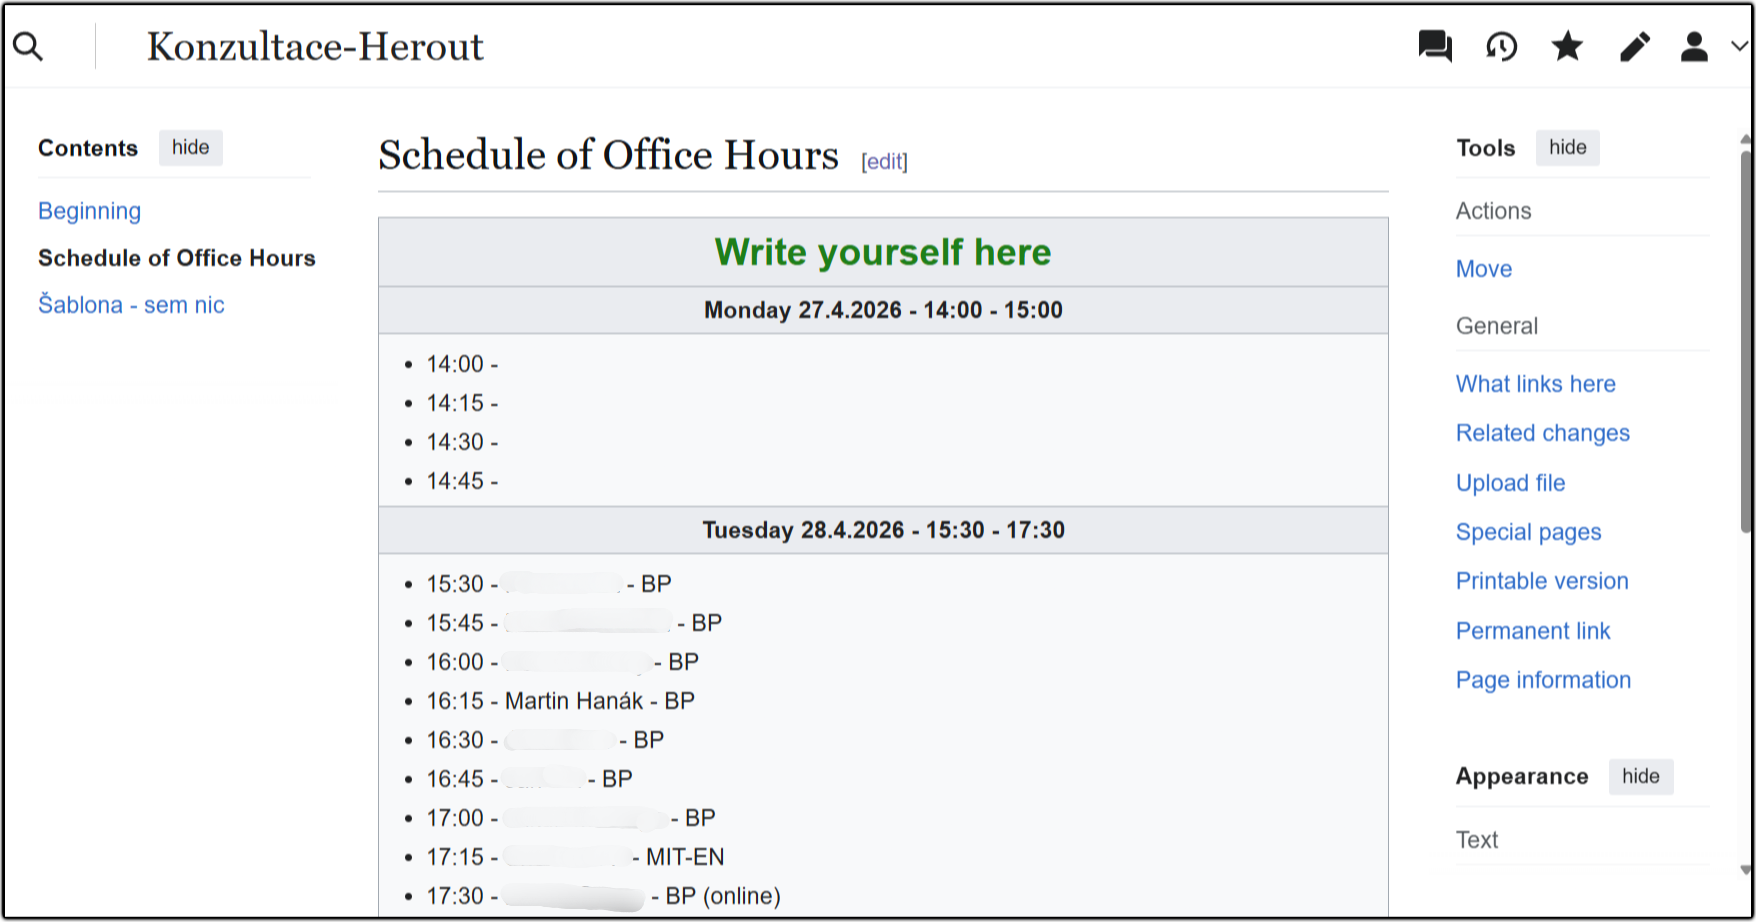
\includegraphics[width=1\textwidth]{obrazky-figures/analyza-wikimerlin.png}
    \caption{Používateľské rozhranie systému Wiki@Merlin s rezervačnými blokmi. Ako príklad je zobrazený reálny rezervačný formulár konzultačných hodín prof. Ing. Adama Herouta, Ph.D.}
    \label{fig:wikimerlin}
\end{figure}
\begin{figure}[t]
    \centering
    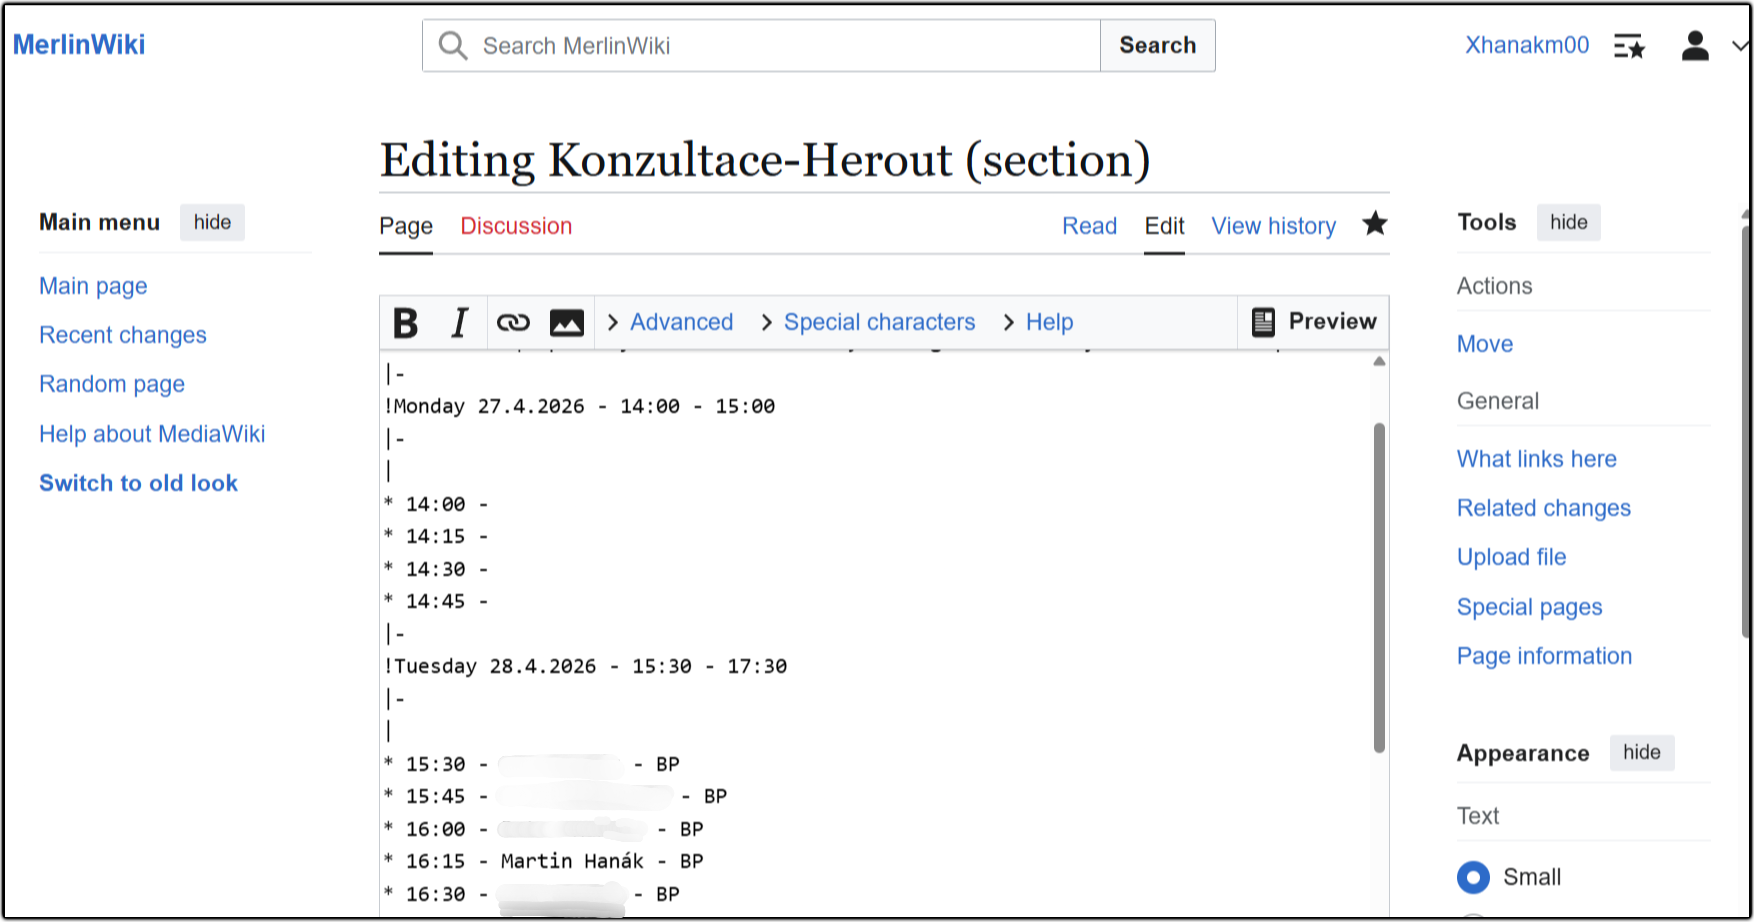
\includegraphics[width=1\textwidth]{obrazky-figures/analyza-wikimerlin-edit-mode.png}
    \caption{Editačný mód systému Wiki@Merlin s ukážkou rezervácie konzultačného slotu prostredníctvom priamej editácie textového dokumentu.}
    \label{fig:wikimerlin-edit}
\end{figure}

\subsection{Systém pre správu diplomových prác (Diplomky FIT)}
Novšou a sofistikovanejšou alternatívou je fakultný systém Diplomky FIT\footnote{Diplomky FIT – Dostupné na: \url{https://www.diplomkyfit.cz/}}. Oproti systému Wiki@Merlin predstavuje tento nástroj výrazný posun vpred. Jeho hlavnou výhodou je webové rozhranie a práca so štruktúrovanou databázou, vďaka čomu sú rezervácie termínov a správa dát prehľadnejšie a chránené proti neoprávnenej manipulácii inými používateľmi.

Napriek týmto výhodám má systém z pohľadu modernej prístupnosti aj svoje limity. Prvým z nich je chýbajúca natívna mobilná aplikácia. 
Hoci webové rozhranie je responzívne, mobilná aplikácia by používateľom poskytla vyšší komfort, rýchlejší prístup a lepšiu integráciu s mobilným operačným systémom bez nutnosti otvárať prehliadač.

Druhým výrazným obmedzením je striktná politika autentifikácie. Prihlásenie do tohto systému je podmienené výlučne vlastníctvom univerzitnej e-mailovej adresy s doménou \textbf{@fit.vutbr.cz}. Napríklad adresy v tvare \textbf{xlogin00@stud.fit.vut.cz} nie sú systémom akceptované. Tento formát predstavuje prekážku pre študentov, ktorí by pri komunikácii a organizácii stretnutí preferovali využitie svojich osobných e-mailových schránok.

Tretím obmedzením je absencia podpory online konzultácií. Systém umožňuje výlučne rezerváciu termínov osobných stretnutí a neposkytuje žiadnu natívnu integráciu s nástrojmi pre videohovory či vzdialenú komunikáciu. Vyučujúci a študenti, ktorí preferujú alebo vyžadujú online formu konzultácie, sú tak nútení riešiť koordináciu platformy a odkazu na stretnutie mimo systému, čo zbytočne komplikuje celý proces.

\subsection{Google Kalendár}
Okrem špecifických fakultných systémov sa na organizáciu stretnutí využívajú aj globálne komerčné platformy. Jedným z nich je Google Kalendár\footnote{Google Kalendár – online kalendárová služba od spoločnosti Google. Dostupné na: \url{https://calendar.google.com}}. Tento nástroj vyniká technickým spracovaním a vysokou spoľahlivosťou, a tak môže plne vyhovovať používateľom, ktorí preferujú centralizáciu a chcú mať všetky svoje osobné, pracovné aj školské udalosti na jednom mieste.

Hlavnou nevýhodou tohto riešenia v kontexte konzultácií na fakulte je však jeho príliš všeobecné zameranie, ktoré nedokáže vždy plne pokryť špecifické požiadavky vyučujúcich a študentov.

Google Kalendár neumožňuje logické členenie na miestnosti, bloky a sloty. Základné zdieľanie kalendára (kto môže vidieť termíny) je v Google Kalendári bezplatné. Obmedzenie prístupu ku konzultáciám výhradne pre konkrétne e-mailové adresy či vybrané domény – teda overenie, kto môže vykonať rezerváciu – je síce technicky možné, avšak táto funkcia je dostupná len v platených plánoch~\cite{google_appointment_booking}. V bezplatnej verzii teda rezerváciu môže vykonať ktokoľvek, kto disponuje odkazom, čo otvára priestor pre fiktívne rezervácie a blokovanie termínov neoprávnenými osobami.

Ďalšou nevýhodou pre študentov je spôsob zobrazovania obsadenosti. Na rezervačnej stránke Google Kalendára sú zobrazené iba voľné termíny – obsadené sloty nie sú viditeľné. Keďže študenti svoje konzultácie často rušia alebo presúvajú, je pre nich v praxi oveľa výhodnejšie vidieť celý blok vrátane už obsadených slotov. Takýto prehľad im umožňuje sledovať aj plné termíny a prípadne si zapnúť upozornenia pre prípad, že by sa nimi preferovaný slot uvoľnil. 

Kombinácia uvedených obmedzení robí z Google Kalendára nástroj, ktorý síce exceluje ako univerzálne riešenie, avšak pre účely štruktúrovanej správy konzultácií na fakulte poskytuje len nedostatočnú funkčnú podporu.

\begin{figure}[t]
    \centering
    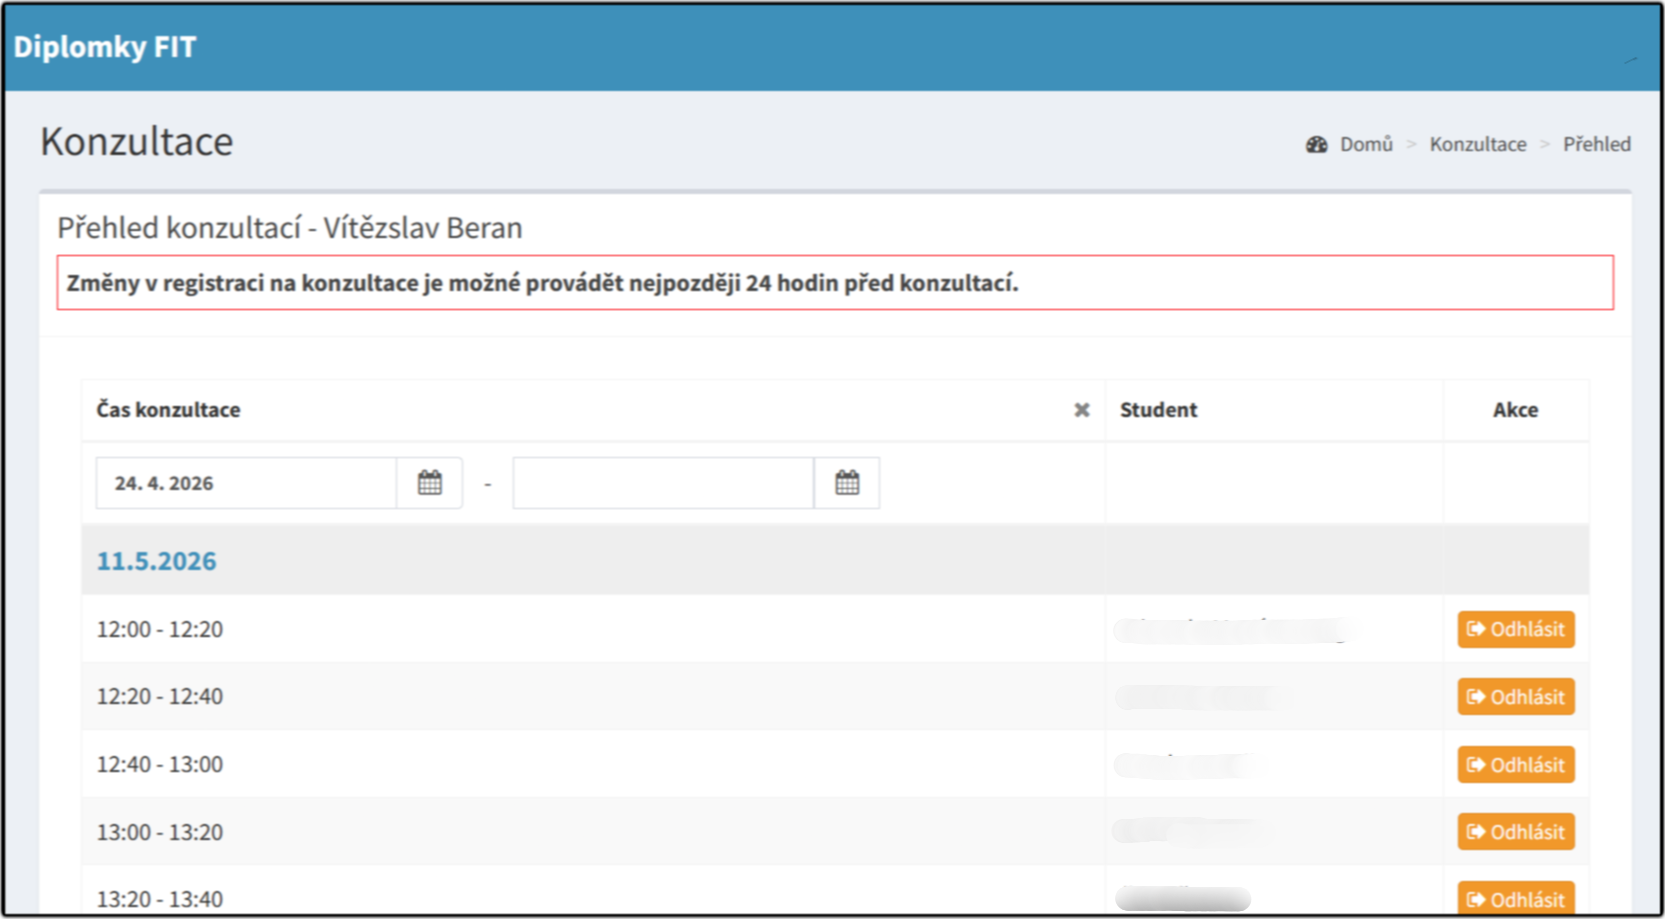
\includegraphics[width=1\textwidth]{obrazky-figures/analyza-diplomky.png}
    \caption{Rozhranie systému Diplomky FIT so zoznamom dostupných 
termínov konzultácií. Ako príklad je zobrazený reálny rezervačný formulár konzultačných hodín doc. Ing. Vítězslava Berana, Ph.D.}
    \label{fig:diplomky}
\end{figure}
\begin{figure}[t]
    \centering
    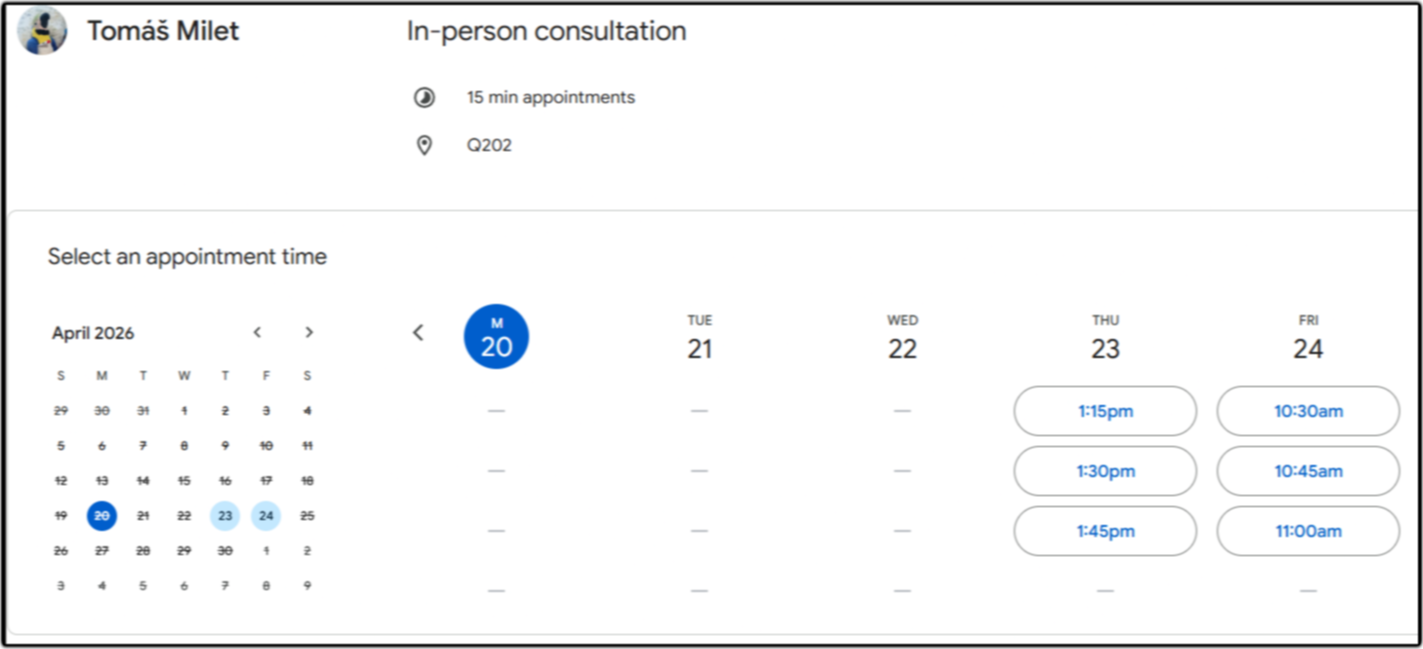
\includegraphics[width=1\textwidth]{obrazky-figures/analyza-google-calendar.png}
    \caption{Rezervačná stránka Google Kalendára zobrazujúca 
výlučne voľné termíny – obsadené sloty nie sú pre návštevníka viditeľné. Ako príklad je zobrazený reálny rezervačný formulár konzultačných hodín Ing. Tomáša Mileta, Ph.D.}
    \label{fig:googlecalendar}
\end{figure}
\subsection{Microsoft Excel}
Ďalším príkladom globálneho komerčného riešenia, ktoré sa v praxi využíva na správu konzultačných hodín, je tabuľkový editor Microsoft Excel\footnote{Microsoft Excel – tabuľkový editor od spoločnosti Microsoft. Dostupné na: \url{https://www.microsoft.com/microsoft-365/excel}}. Podobne ako pri Wiki@Merlin, aj toto riešenie sa spolieha na disciplínu a pozornosť samotných používateľov, keďže neposkytuje žiadnu ochranu jednotlivých záznamov. Každý používateľ s oprávnením na úpravu súboru môže omylom alebo zámerne prepísať či vymazať záznamy iných študentov, čo vystavuje celý harmonogram konzultácií riziku neúmyselného poškodenia alebo straty dát.

Z hľadiska prístupu platí, že zdieľaný excelový súbor býva typicky uložený na platforme Microsoft OneDrive alebo SharePoint, ktorých prístup je vo fakultnom prostredí viazaný na školský účet.

Ovládanie mobilnej aplikácie Microsoft Excel pri práci s rezervačnými tabuľkami je menej pohodlné. Keďže tabuľky bývajú rozsiahle v oboch osiach, používateľ je nútený posúvať zobrazenie horizontálne aj vertikálne, aby získal úplný prehľad o dostupných termínoch. Orientácia v takomto prostredí na malom displeji smartfónu je nepohodlná a zvyšuje riziko neúmyselných chýb pri editácii.

Čo sa týka notifikácií, Microsoft Excel v kombinácii s OneDrive alebo SharePoint umožňuje prijímať e-mailové upozornenia pri zmene súboru prostredníctvom funkcie \textit{Alert Me} alebo automatizovaných tokov v nástroji Power Automate~\cite{microsoft_sharepoint_alerts}. Tieto notifikácie sú však dostupné len na úrovni celého súboru – systém informuje o tom, že bol súbor zmenený, nie o tom, ktorý konkrétny blok bol upravený.

Napriek týmto obmedzeniam Excel ako rezervačný nástroj funguje – je široko dostupný a pre jednoduché scenáre postačuje. Ide však o všeobecný nástroj, ktorý nebol navrhnutý pre účely štruktúrovanej správy konzultácií, a preto chýbajú funkcie ako logické členenie na miestnosti a bloky alebo automatická ochrana rezervácií.

\begin{figure}[t]
    \centering
    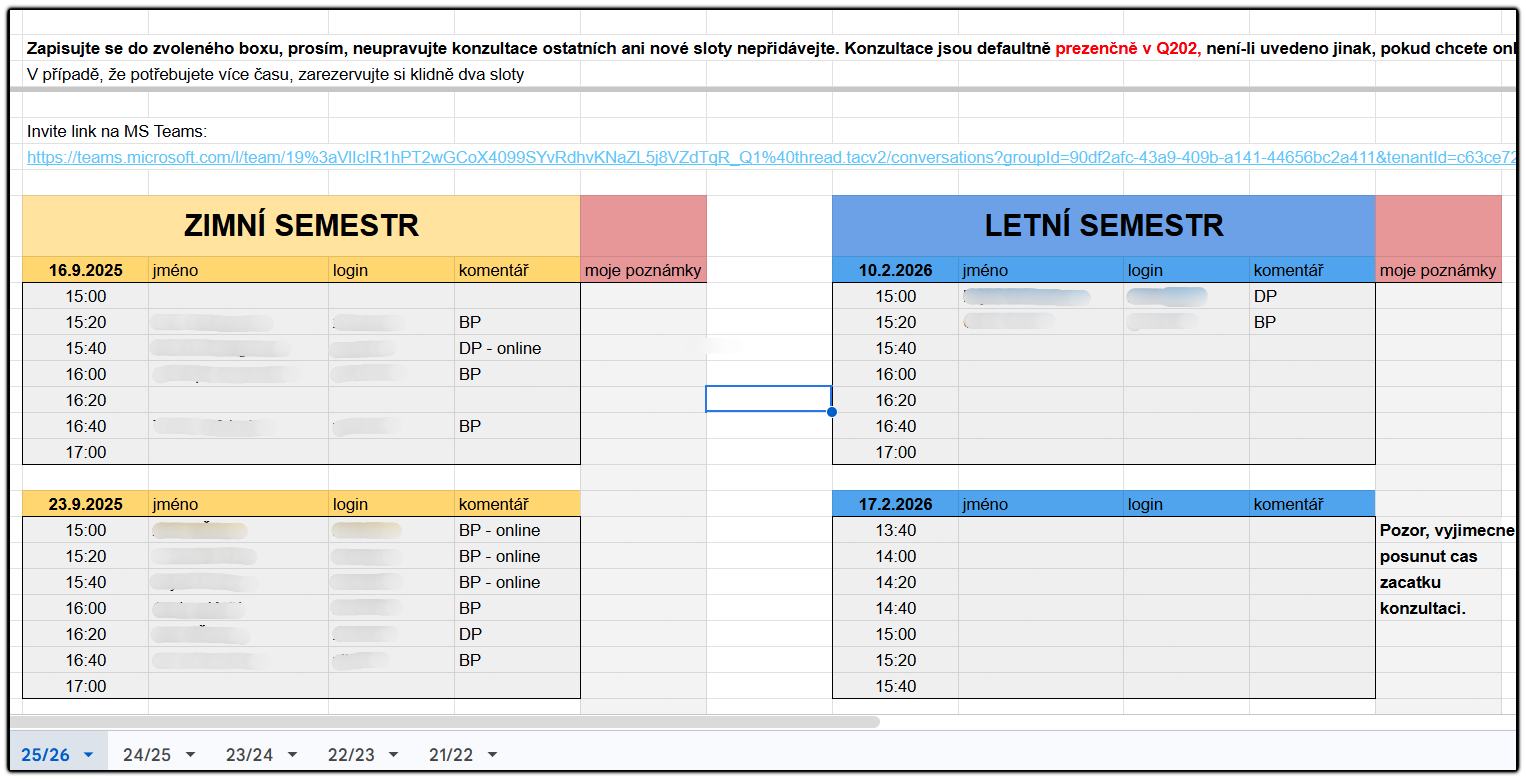
\includegraphics[width=1\textwidth]{obrazky-figures/analyza-excel.png}
    \caption{Rezervačná stránka Excel. Ako príklad je zobrazený excel dokument Ing. Michala Vlnasa.}
    \label{fig:excel}
\end{figure}
\subsection{Zhodnotenie a motivácia pre vlastné riešenie}

\begin{table}[t]
\centering
\caption{Porovnanie existujúcich rezervačných systémov.}
\label{tab:porovnanie}
\resizebox{\linewidth}{!}{%
\begin{tabular}{|l|c|c|c|c|}
\hline
\textbf{Vlastnosť} & \textbf{Wiki@Merlin} & \textbf{Diplomky FIT} & \textbf{Google Kalendár} & \textbf{Excel} \\
\hline
Ochrana rezervácií                 & \texttimes & \checkmark & \checkmark & \texttimes \\
\hline
Mobilná aplikácia                  & \texttimes & \texttimes & \checkmark & \checkmark \\
\hline
Kontrola prístupu                  & \checkmark & \checkmark & $\circ$    & \checkmark \\
\hline
Viditeľnosť obsadených slotov      & \checkmark & \checkmark & \texttimes & \checkmark \\
\hline
E-mailové notifikácie              & \texttimes & \checkmark & \checkmark & $\bullet$  \\
\hline
Online stretnutia              & \checkmark & \texttimes & \checkmark & \checkmark   \\
\hline
\end{tabular}}
\smallskip
\par\footnotesize{$^\circ$~Overenie e-mailu pred rezerváciou (obmedzenie prístupu) je dostupné len v platených plánoch. Základné zdieľanie kalendára je bezplatné.
\\\quad$^\bullet$~Notifikácia len na úrovni celého súboru, nie jednotlivých zmien.}
\end{table}

Tabuľka~\ref{tab:porovnanie} sumarizuje kľúčové vlastnosti analyzovaných systémov. Z porovnania vyplýva, že hoci každý z nich pokrýva určitú podmnožinu požadovanej funkcionality, žiadny nespĺňa všetky potreby súčasne. Systém Wiki@Merlin je technologicky zastaraný a nezabezpečuje ochranu dát pred nežiaducou modifikáciou. Systém Diplomky FIT síce rieši integritu dát, ale chýba mu mobilná podpora a možnosť online konzultácií. Globálne riešenie Google Kalendár zasa nezohľadňuje špecifické potreby fakulty a v bezplatnej verzii neposkytuje dostatočnú kontrolu prístupu. Microsoft Excel síce ponúka
zdieľanú editáciu, avšak ako univerzálny tabuľkový editor
postráda ochranu jednotlivých rezervácií a neposkytuje štruktúrovaný prehľad vhodný
pre správu konzultačných hodín. Tieto nedostatky tvoria priamu motiváciu pre vývoj vlastnej aplikácie.

\section{Špecifikácia požiadaviek na systém}
Požiadavky na systém vychádzajú z analýzy existujúcich riešení a definovaných cieľov práce. Rozdeľujú sa na funkčné – čo musí systém vedieť robiť – a nefunkčné – akými vlastnosťami musí disponovať.
\subsection{Funkčné požiadavky}
Používateľské roly nie sú viazané na profesijné označenie, ale na vzťah k miestnosti. Jeden používateľ tak môže byť v jednej miestnosti Majiteľom a v inej Návštevníkom. To znamená, že rovnaký používateľ – napríklad doktorand, ktorý vedie vlastné konzultácie za cvičenia, ale zároveň chodí na konzultácie k svojmu školiteľovi – by v systéme nemohol byť súčasne učiteľom aj študentom, keby sme roly nazvali „Teacher“ a „Student“. Preto sú roly definované výlučne vzťahom ku konkrétnej miestnosti: v jednej miestnosti vystupuje ako jej Majiteľ (zodpovedá učiteľovi), v inej len ako Návštevník (zodpovedá študentovi).
\begin{itemize}
\item \textbf{Autentifikácia:} Registrácia a prihlásenie prebiehajú cez e-mailovú adresu a jednorazový OTP kód. Nový používateľ nemá prístup k žiadnym dátam, kým ho Majiteľ nepridá do svojej miestnosti.
\item \textbf{Správa miestností (Majiteľ):} Vytváranie, úprava a mazanie konzultačných miestností.
\item \textbf{Správa blokov a slotov (Majiteľ):} Vytváranie, úprava a mazanie časových blokov a slotov v rámci nich.
\item \textbf{Riadenie prístupu (Majiteľ):} Správa zoznamu povolených e-mailových adries pre každú miestnosť.
\item \textbf{Rezervácia (Návštevník):} Prezeranie dostupných miestností, blokov a slotov a rezervovanie voľného slotu s možnosťou pridania textovej poznámky popisujúcej dôvod stretnutia.
\item \textbf{Zrušenie rezervácie (Návštevník):} Návštevník môže zrušiť vlastnú rezerváciu. Ak ju zruší neskoro, systém ho na túto skutočnosť upozorní.
\item \textbf{Nastavenia a GDPR:} Používateľ si môže prispôsobiť vizuálny motív a skryť svoje meno voči ostatným používateľom.
\item \textbf{E-mailové notifikácie:} Automatické upozornenia obom stranám pri zmenách, pokiaľ to používateľ povolí v nastaveniach.
\item \textbf{Prehľad pripojených používateľov (Majiteľ):} 
Majiteľ má k dispozícii prehľad o tom, ktorí 
návštevníci sú v danej miestnosti pripojení.
\end{itemize}
\subsection{Nefunkčné požiadavky}
\begin{itemize}
\item \textbf{Multiplatformová podpora:} Aplikácia musí byť plne funkčná na Androide aj iOS z jedinej kódovej základne (Flutter).
\item \textbf{Bezpečnosť:} Prístup k dátam je povolený výlučne autentifikovaným používateľom. Spojenie so serverom musí byť udržiavané bezpečným mechanizmom bez nutnosti opakovane zadávať prihlasovacie údaje, ak si to používateľ praje.
\item \textbf{Odozva (Optimistic UI):} Pri bežných interakciách (rezervácia, zrušenie) aplikácia reaguje vizuálne okamžite a potvrdenie prebehne asynchrónne na pozadí. Ak zmena nebude úspešná, aplikácia sa vráti do pôvodného stavu. Blokujúce načítavacie obrazovky sú vyhradené len pre nevyhnutné operácie ako napríklad počiatočné stiahnutie dát.
\item \textbf{Používateľské rozhranie:} UI musí rešpektovať moderné dizajnové štandardy a umožňovať intuitívnu navigáciu.
\end{itemize}
\subsection{Modelovanie prípadov použitia (Use Cases)}
Na základe definovaných požiadaviek bol zostavený diagram prípadov použitia (Obrázok~\ref{fig:usecase}), ktorý vizualizuje interakcie aktérov so systémom.
Vzťah medzi Majiteľom a Návštevníkom je definovaný generalizáciou – Majiteľ dedí všetky oprávnenia Návštevníka a navyše disponuje právami na správu rezervačného priestoru. Každý používateľ musí prejsť autentifikáciou. Relácia \textbf{<<include>>} definuje, že operácie \uv{Zaregistrovať sa} aj \uv{Prihlásiť sa} povinne zahŕňajú krok \uv{Overiť pomocou OTP}.
Návštevník má k dispozícii funkcie prezerania miestností, blokov a slotov, pričom relácia \textbf{<<extend>>} umožňuje voliteľné správanie – nastavenie upozornenia na blok, pridanie poznámky k rezervácii či upozornenie pri rušení rezervácie na poslednú chvíľu.
Z pohľadu Majiteľa diagram definuje administrátorské funkcie: \uv{Spravovať miestnosť}, \uv{Spravovať blok} a \uv{Spravovať slot}, pričom \uv{Riadenie prístupu k miestnosti} (zahrnuté cez \textbf{<<include>>}) umožňuje obmedziť prístup na konkrétne e-mailové adresy alebo celé domény.

\begin{figure}[t]
    \centering
    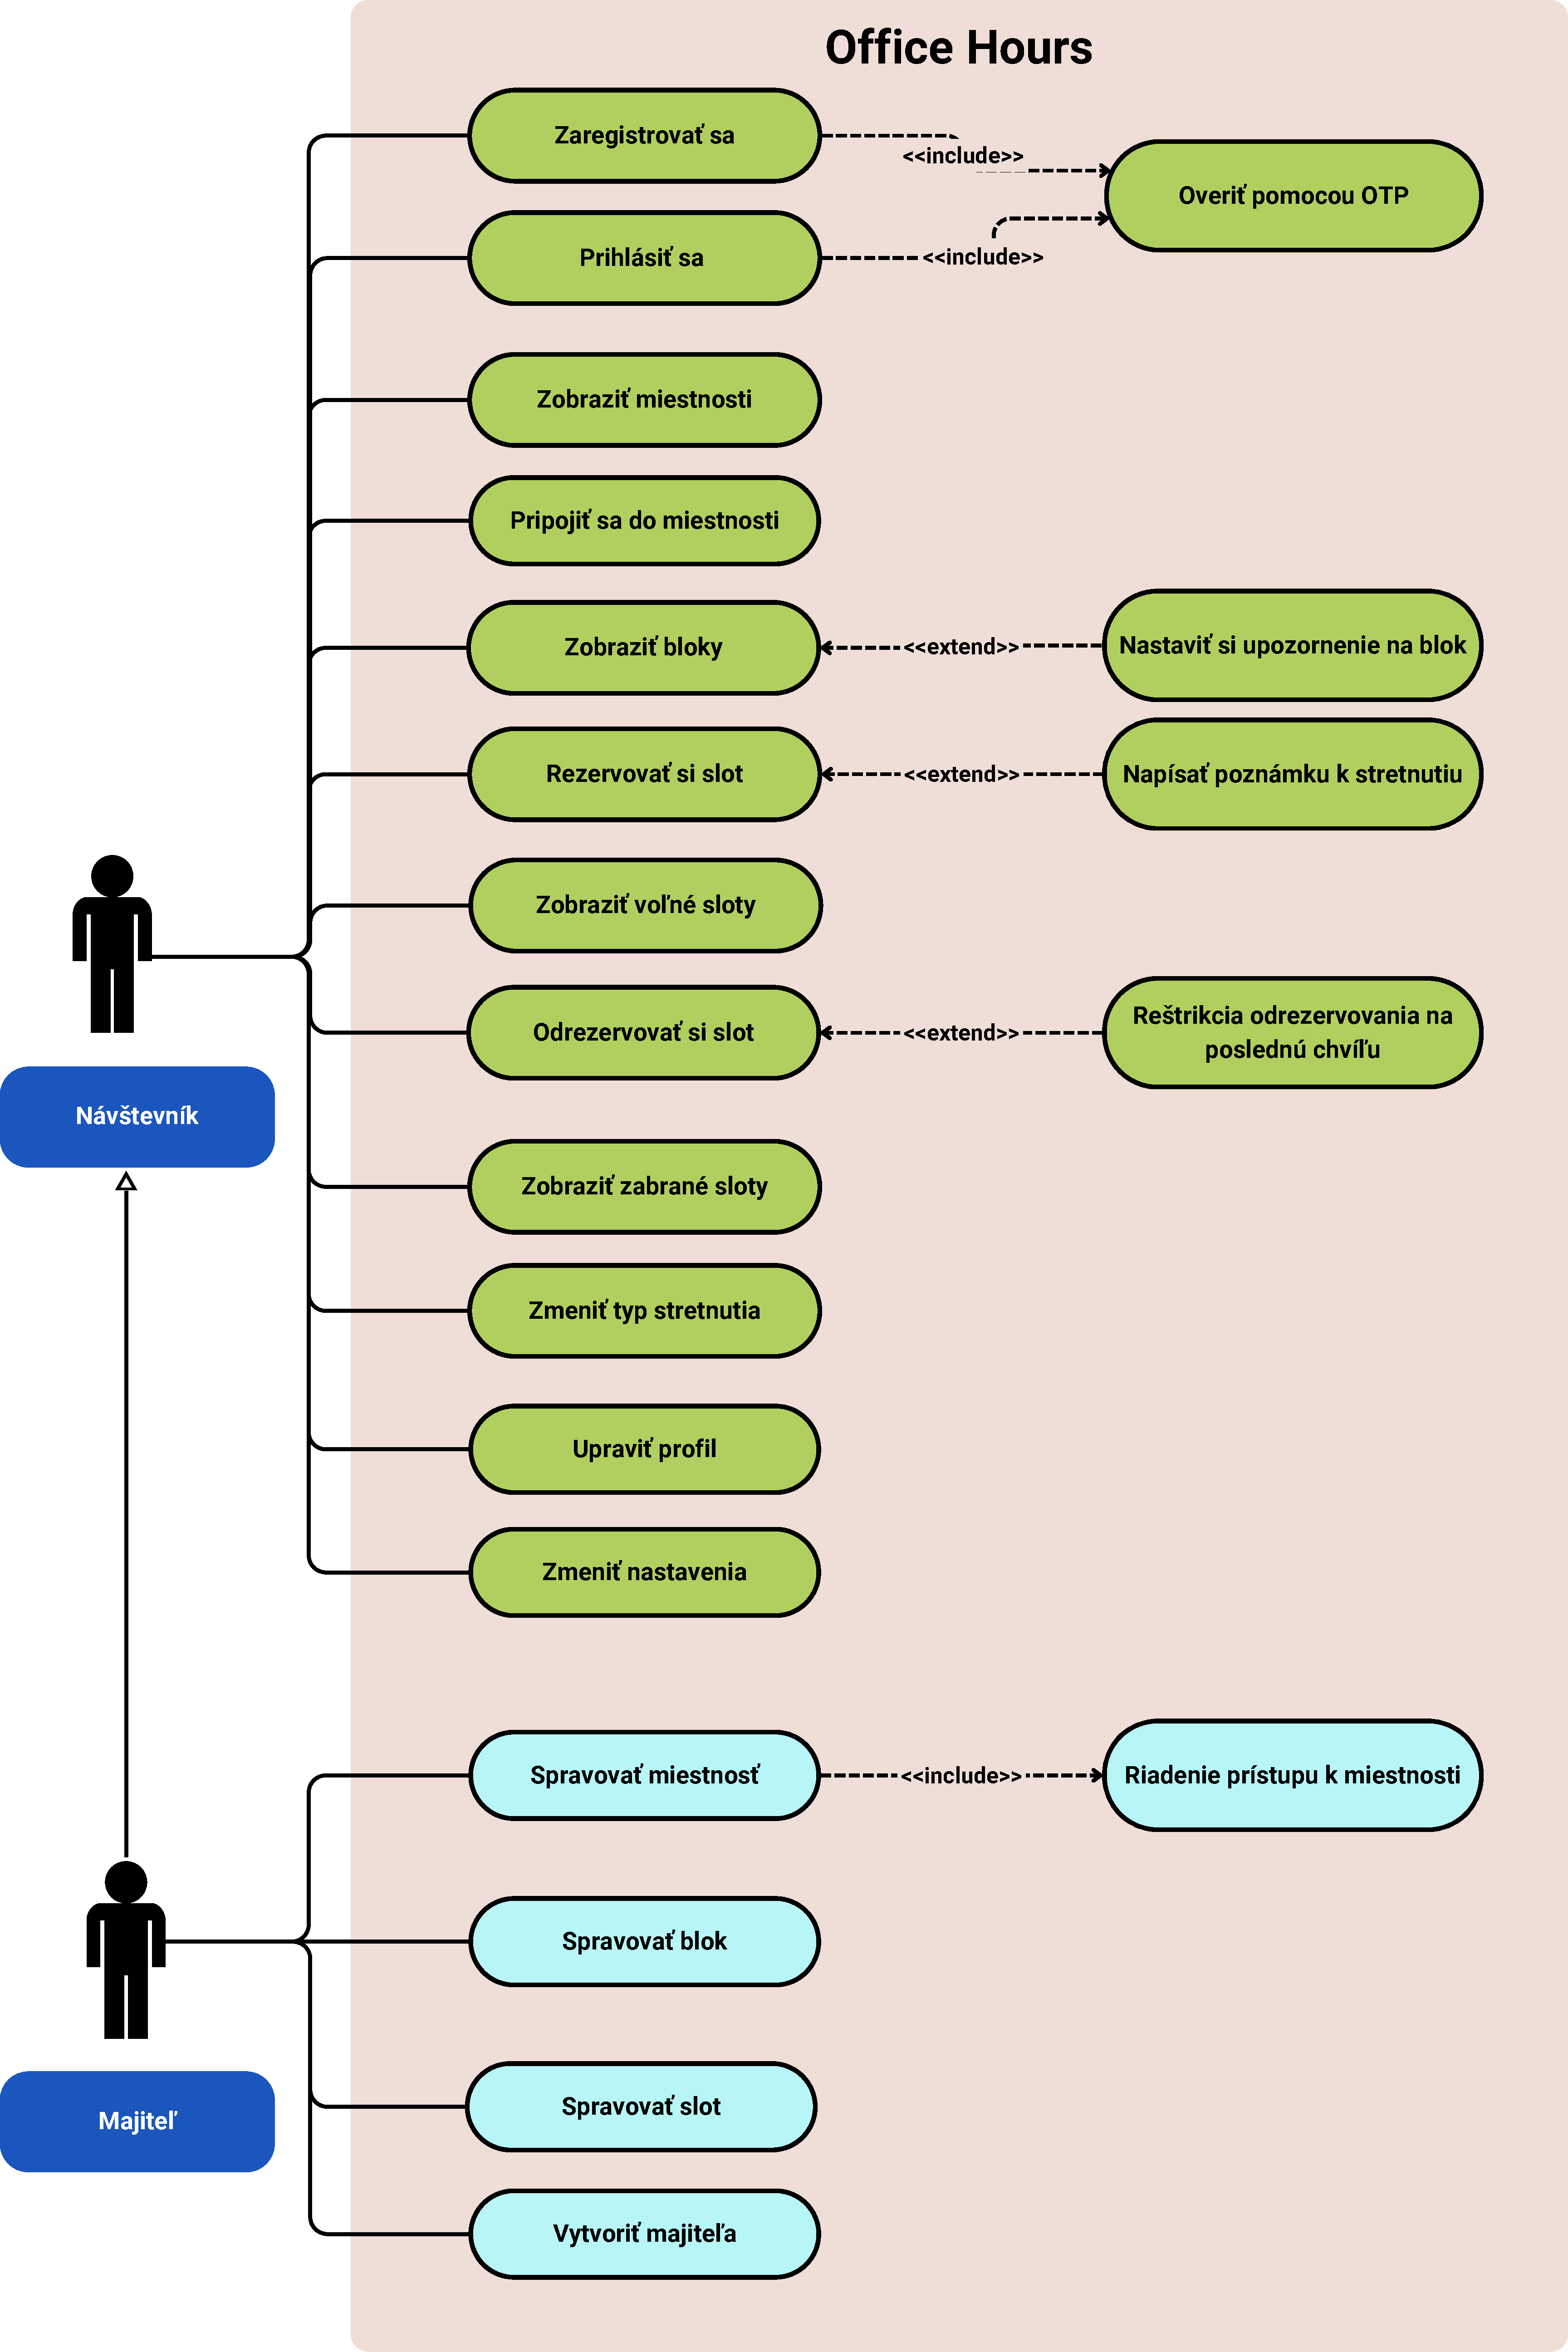
\includegraphics[width=0.9\textwidth]{obrazky-figures/analyza-usecasediagram.pdf}
    \caption{Diagram prípadov použitia aplikácie Office Hours zobrazujúci interakcie
dvoch hlavných aktérov – Návštevníka a Majiteľa.}
    \label{fig:usecase}
\end{figure}